\clearpage
\section{Nuisance Parameters Fit\label{app:prePostFit}}

A maximum likelihood fit to the asimov dataset is performed for all signal models. 
The results for the most sensitive category for a sample signal model (T1bbbb 1500,100) and for 
a 10, 25, 50, and 100\% template variation in the final bin are shown in Fig.~\ref{fig:prePost}. 
The nuisances on the transfer factors (as well as the signal acceptance) agree 
well with their pre-fit values. This is expected as these nuisances are uncorrelated 
and derived from the statistical precision of control samples, which should be
higher than that in the signal region. For an uncertainty of greater than 10\%
on the last bin the width of the template systematic is reduced by the fit.
The information in the signal region is sufficient in this case
to constrain the template variation. 

\begin{figure}[h!]
 \begin{center}  
  \subfigure[Shape Variation of 100\%]{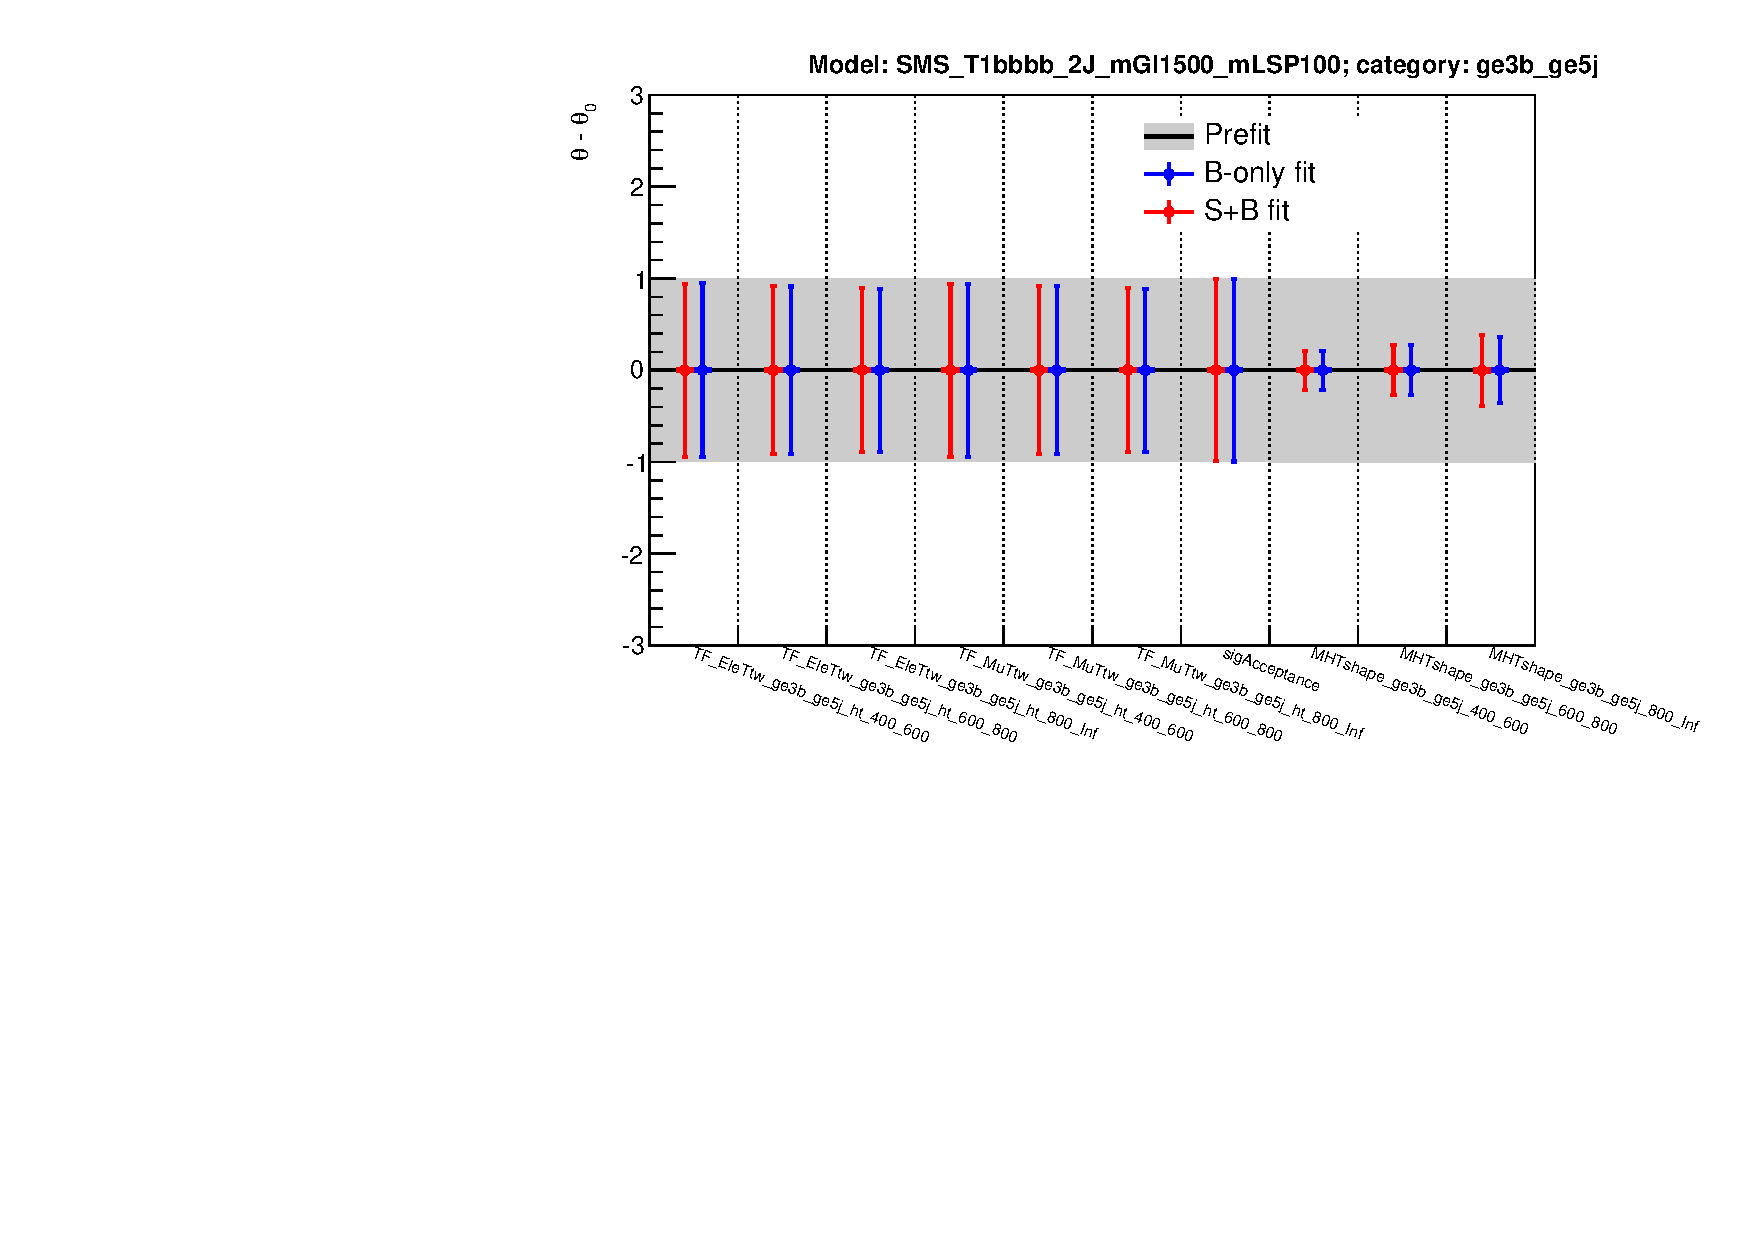
\includegraphics[width=0.5\textwidth]{figures/prePostFit/nuisanceDiagnostic100/nuisances_SMS_T1bbbb_2J_mGl1500_mLSP100.pdf}} ~~
  \subfigure[Shape Variation of 50\%]{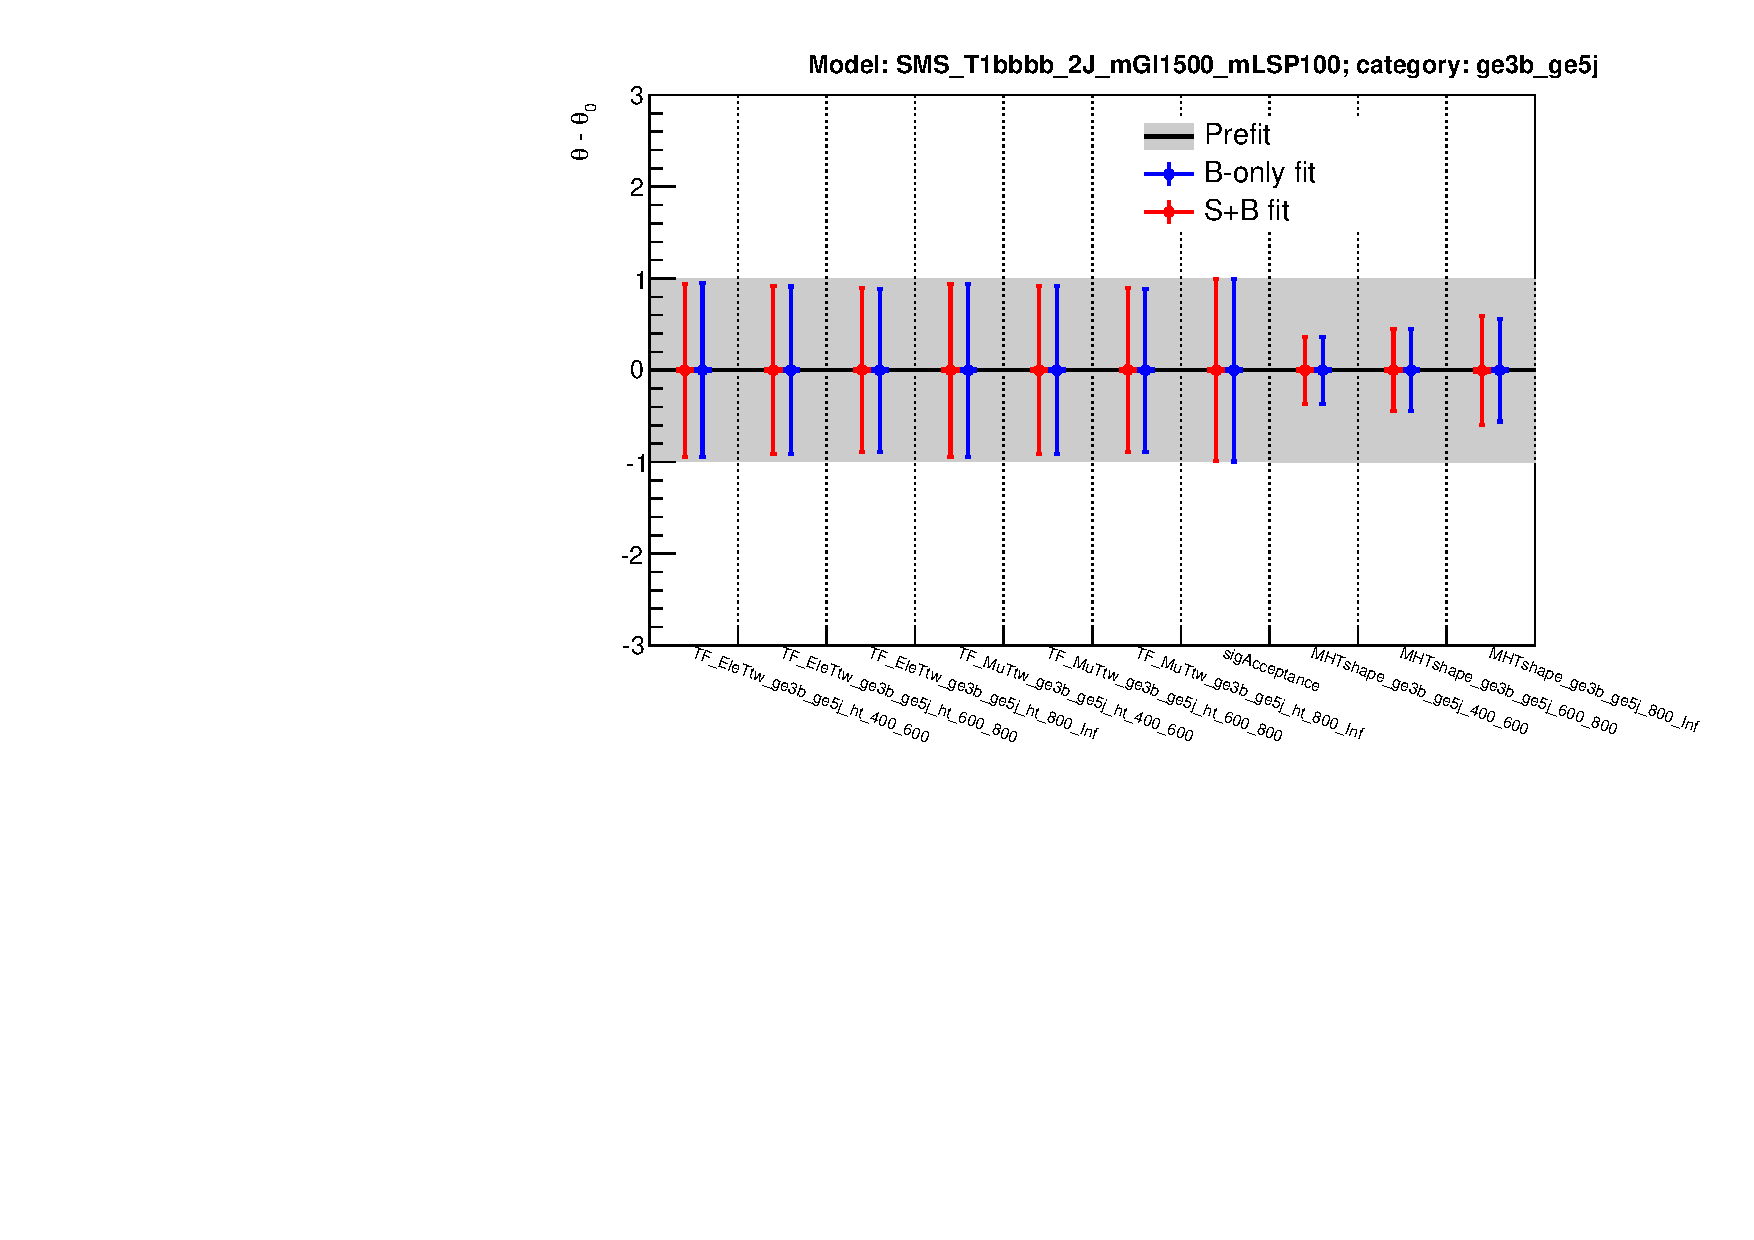
\includegraphics[width=0.5\textwidth]{figures/prePostFit/nuisanceDiagnostic50/nuisances_SMS_T1bbbb_2J_mGl1500_mLSP100.pdf}} ~~ \\
  \subfigure[Shape Variation of 25\%]{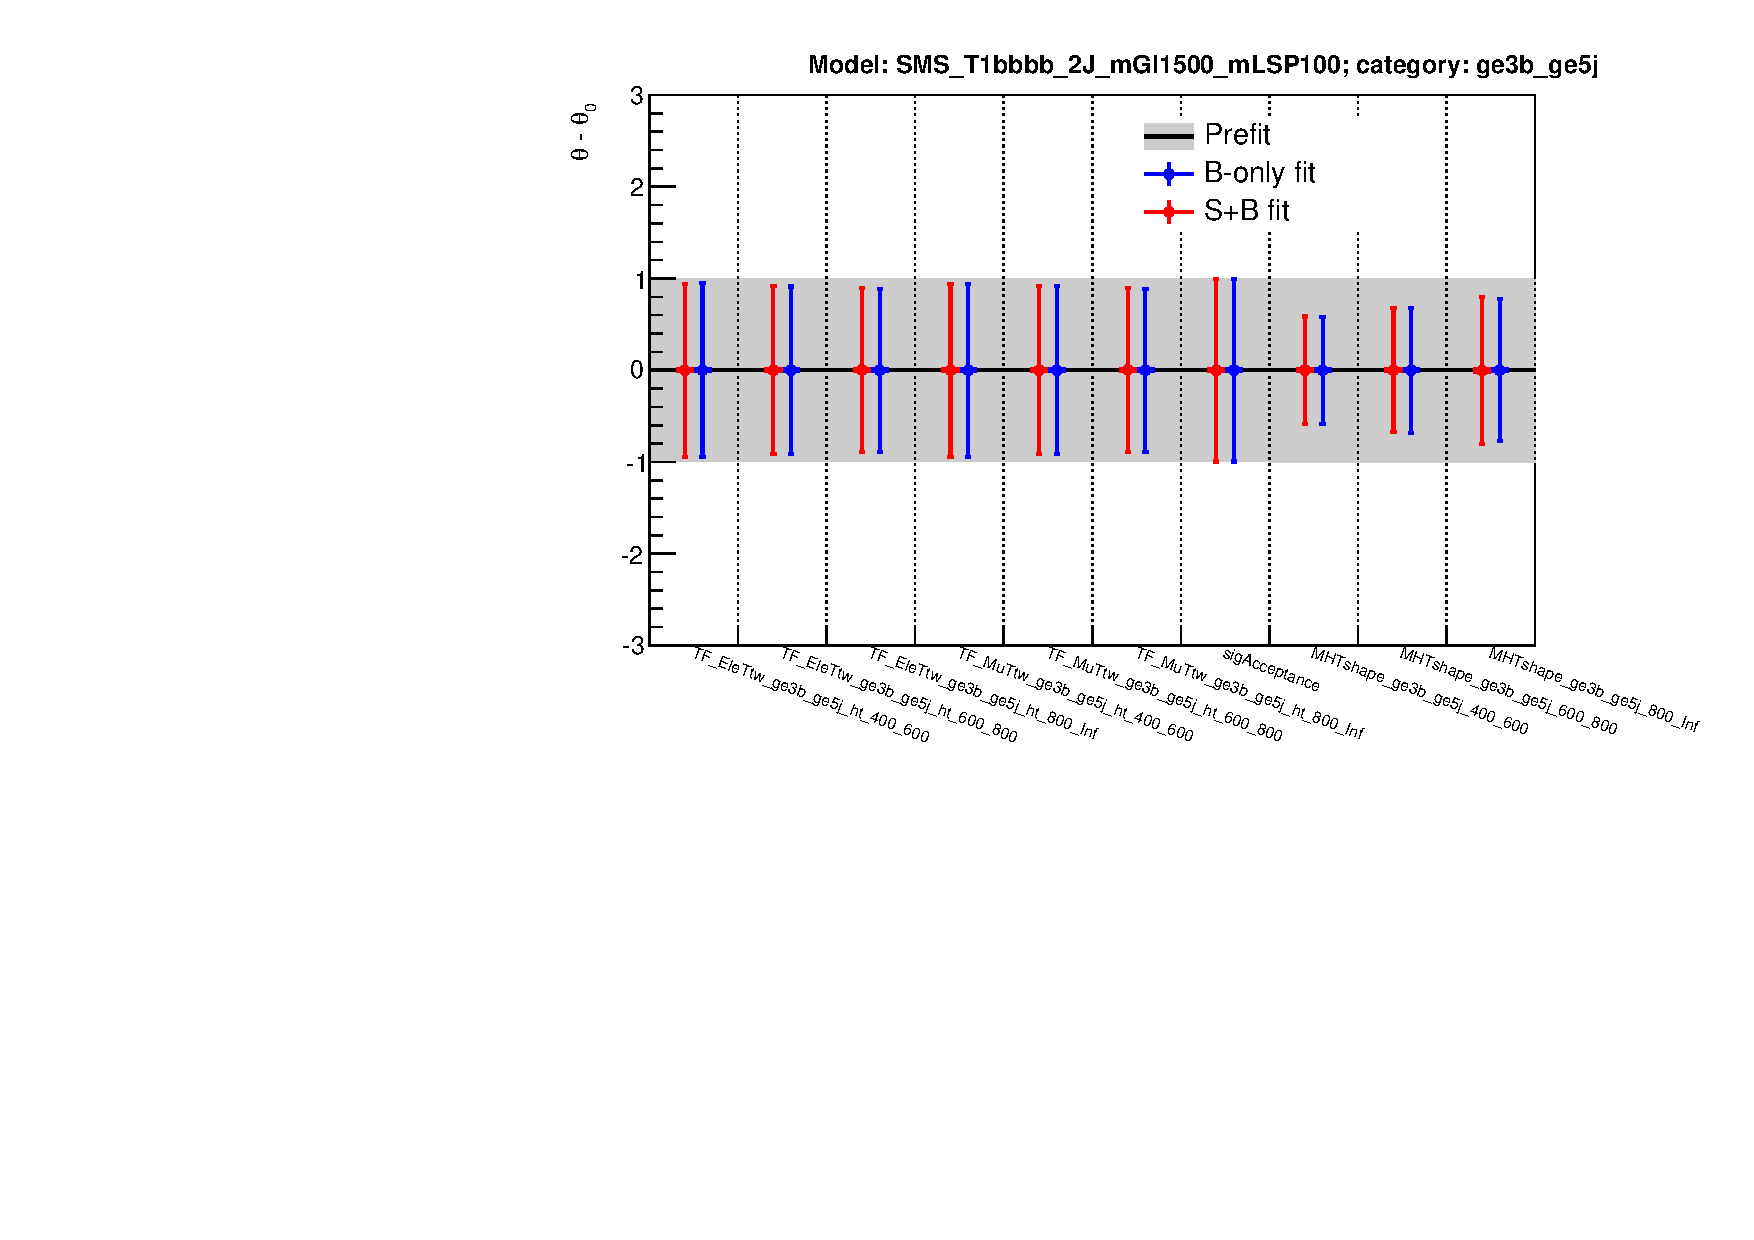
\includegraphics[width=0.5\textwidth]{figures/prePostFit/nuisanceDiagnostic25/nuisances_SMS_T1bbbb_2J_mGl1500_mLSP100.pdf}} ~~
  \subfigure[Shape Variation of 10\%]{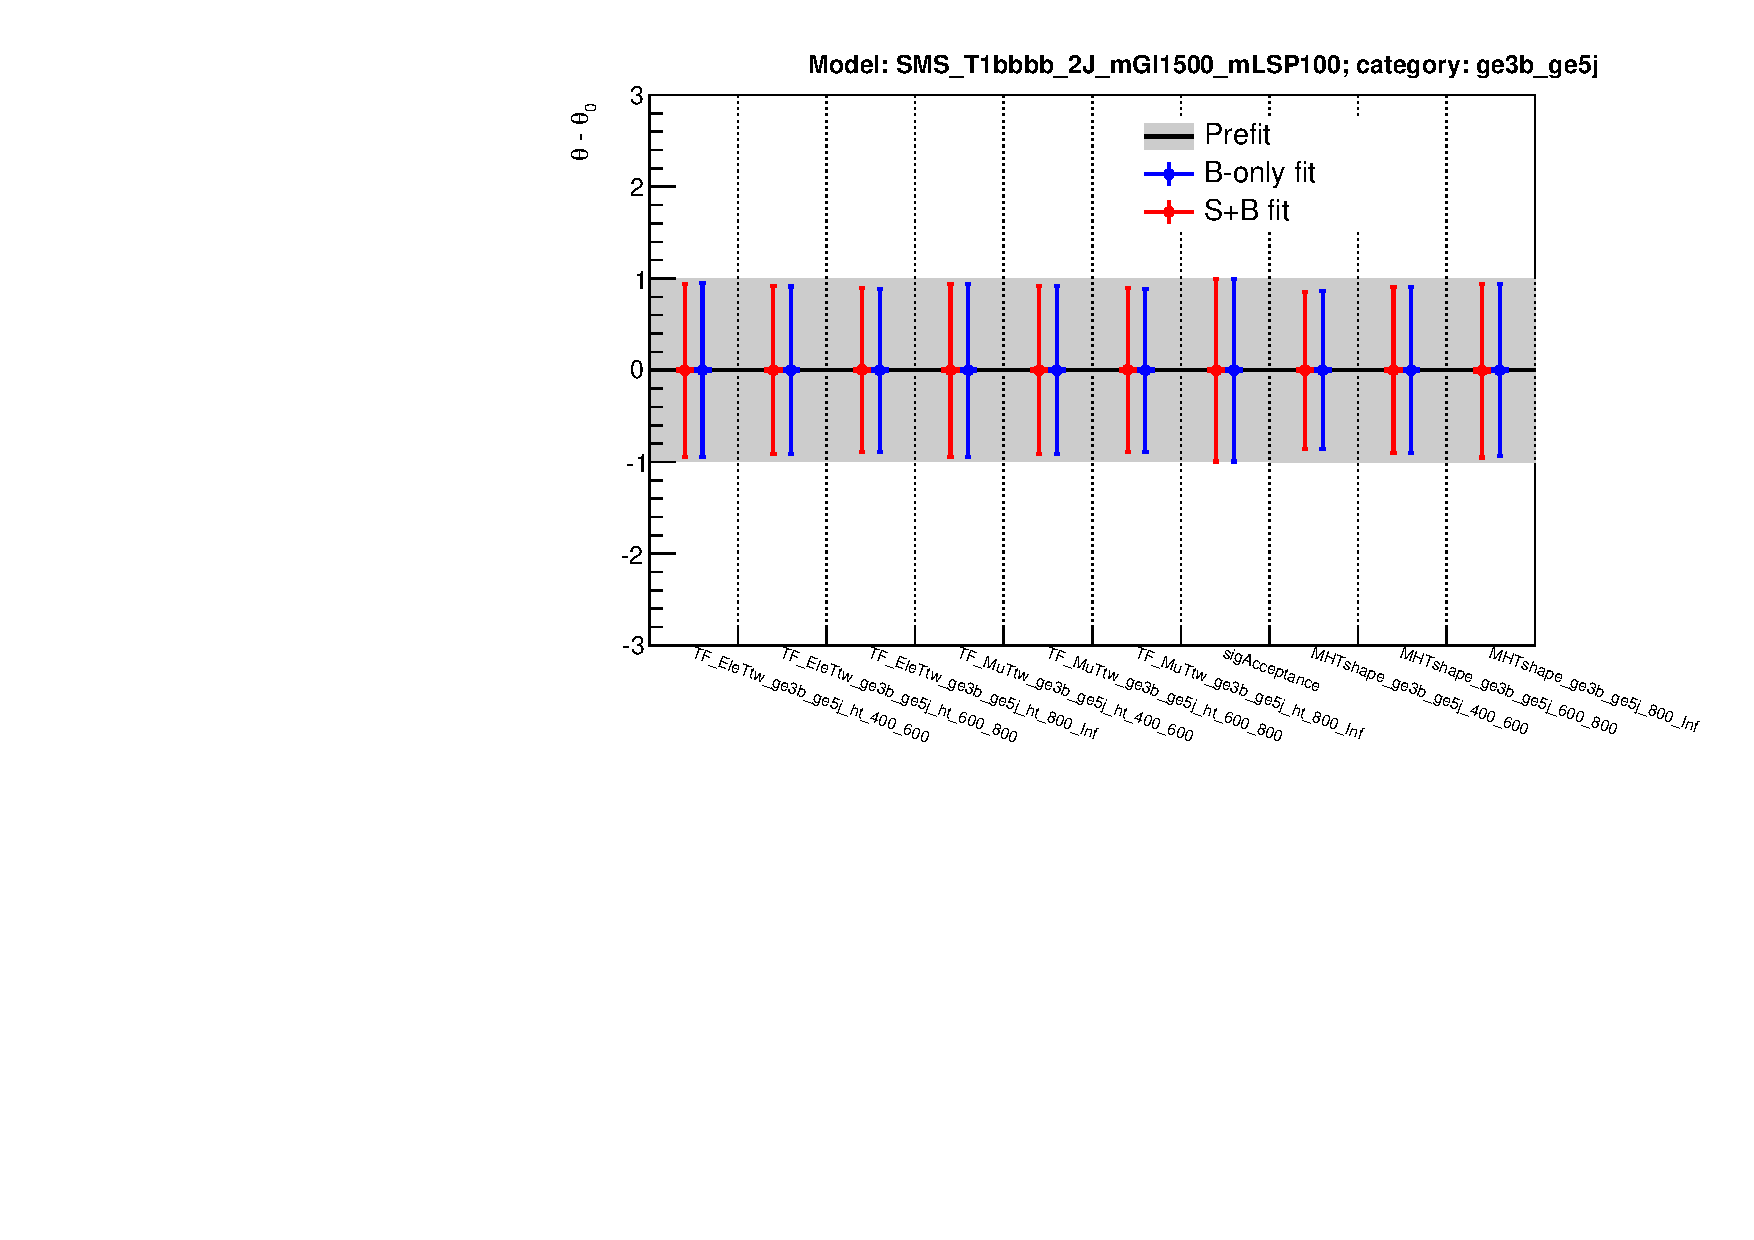
\includegraphics[width=0.5\textwidth]{figures/prePostFit/nuisanceDiagnostic10/nuisances_SMS_T1bbbb_2J_mGl1500_mLSP100.pdf}} \\
  \caption{Effect of the fit on the nuisances for the most sensitive category of T1bbbb 1500, 100. The only substantial difference between pre and post fit is seen in the shape}
  \label{fig:prePost}
 \end{center}
\end{figure}          
